%
% 公立はこだて未来大学卒業研究中間報告書[全コース対応版]
%
%         ファイル名:"sample.tex"
%
\documentclass[11pt]{ujarticle}
\usepackage{funinfosys}
\usepackage{url}
\usepackage[dvipdfmx]{graphicx}

\author{% 
b1020036 中川匠海\\指導教員 : 松原克弥
}
\course{Information Systems Course}

\title{キャンパスDX に向けた学務情報のオープンデータ化}
\etitle{Open Data Initiatives for Academic Affairs Information in Preparation for Campus Digital Transformation (DX)}
\eauthor{Takumi Nakagawa}
\abstract{今日の大学ではLearning Management System(LMS)や教務システムなど、目的に応じて複数のシステムを組み合わせたICT学習支援環境を構築している.しかし、複数のシステムに情報が分散していることや、Webサイトやメール等の限られたアクセス手段しか提供されないことで、学生に対する「学務情報への到達容易性」が課題となっている.
\\ 本研究では、未来大にて使用されている複数のシステムで、それぞれ異なる形式で分散管理されている学務情報(休講、補講、教室変更、振替連絡、課題〆切、教室空き情報など)をスクレイピング技術等を用いて収集し、モバイルアプリなどで活用できるようオープンデータ化し、スマートフォンやSNSなどの情報アクセス媒体になれた「デジタルネイティブ世代」の学生に適した学習支援の実現を目指す.}
\keywords{キャンパスDX,オープンデータ,公立はこだて未来大学}
\eabstract{Modern universities employ Learning Management Systems (LMS) and other systems to create comprehensive ICT learning environments. Nonetheless, the dispersion of information across various systems and limited accessibility impede students' easy retrieval of academic information.
\\In this research, conducted at Mirai University, we seek to collect disparate academic data (including class cancellations, supplementary lessons, room changes, notifications, assignment deadlines, and room availability) through scraping technology. By converting this information into open data, we aim to enhance learning support for 'digital native' students accustomed to smartphones and social networks.}
\ekeywords{CampusDX, OpenData, FUN}
\begin{document}
\maketitle
%\vspace*{-.5cm}

\section{背景と目的}

現代の教育界は、テクノロジーの急速な進展に伴い、その運営方法と学習環境に著しい変化を見せている。全国的に観察すると、キャンパスのデジタルトランスフォーメーション(以降キャンパスDX)が加速しており、リモート授業、デジタル教材、オンライン評価、データ分析など、教育のデジタル化は急速に進行している。この結果として、学務情報へのアクセス性や柔軟性が大幅に向上しているが、新たな課題も顕在化している。

未来大では、教育プロセスの多くがデジタル化されている一方、重要な学務情報が複数のWebサイトに分散しており、情報へのアクセスの困難さが問題となっている。具体的に、学生が必要とする情報は、教務システム(Student)、LMS(HOPE)、情報ライブラリサイト、未来大公式ホームページなど、異なるプラットフォームに散在しています。これにより、学生は必要な情報を効率的に検索し、アクセスすることが困難になっており、学習経験に影響を与える可能性があります。

さらに、現行のシステムは学生への情報更新時の能動的な通知機能が欠如している.この状況では、学生は自ら主体的に情報を取得する必要のある"pull型"アプローチとなっている.従って、情報が更新された際にその内容を自動的に学生に伝える"push型"の通知型メカニズムが存在しない現在は、学生が重要な情報の更新を認識しないとう危険性を増大させる要因となっている.これにより、学生の情報アクセスの効率が低下し、学習における不都合を招く可能性が高まっている.

本研究の実現によって、未来台のキャンパスDXはさらに進展し、デジタルネイティブ世代の学生にとって、より効率的で効果的な学習環境が提供されることが期待される.

%目的

そこで本研究の目的は、スクレイピングを用いて未来大の学務情報をオープンデータ化することによる情報到達容易性向上を目的とする.

\section{スクレイピング}

スクレイピングは、Webページから情報を自動で取得・抽出する技術である.

具体的には、WebページのHTMLやXMLデータを解析し、必要な情報をプログラム的に取り出すプロセスを指す.この技術は、多岐にわたる分野で用いられ、特にデータ解析や機械学習の領域でデータ収集手段として注目を浴びている.

スクレイピングな基本的な手法として、まずHTTPリクエストを使用して目的のWebページのデータを取得します.このプロセスは、Webクローラーというプログラムを用いて、自動的に複数のWebページを巡回し、データを収集することが一般的である.得られたデータから特定の情報を抽出するために、DOMパーサーや正規表現などの方法を使用する.これにより、大量のWebページから一貫した形式でデータを収集することが可能となる.

\begin{figure}[h]
	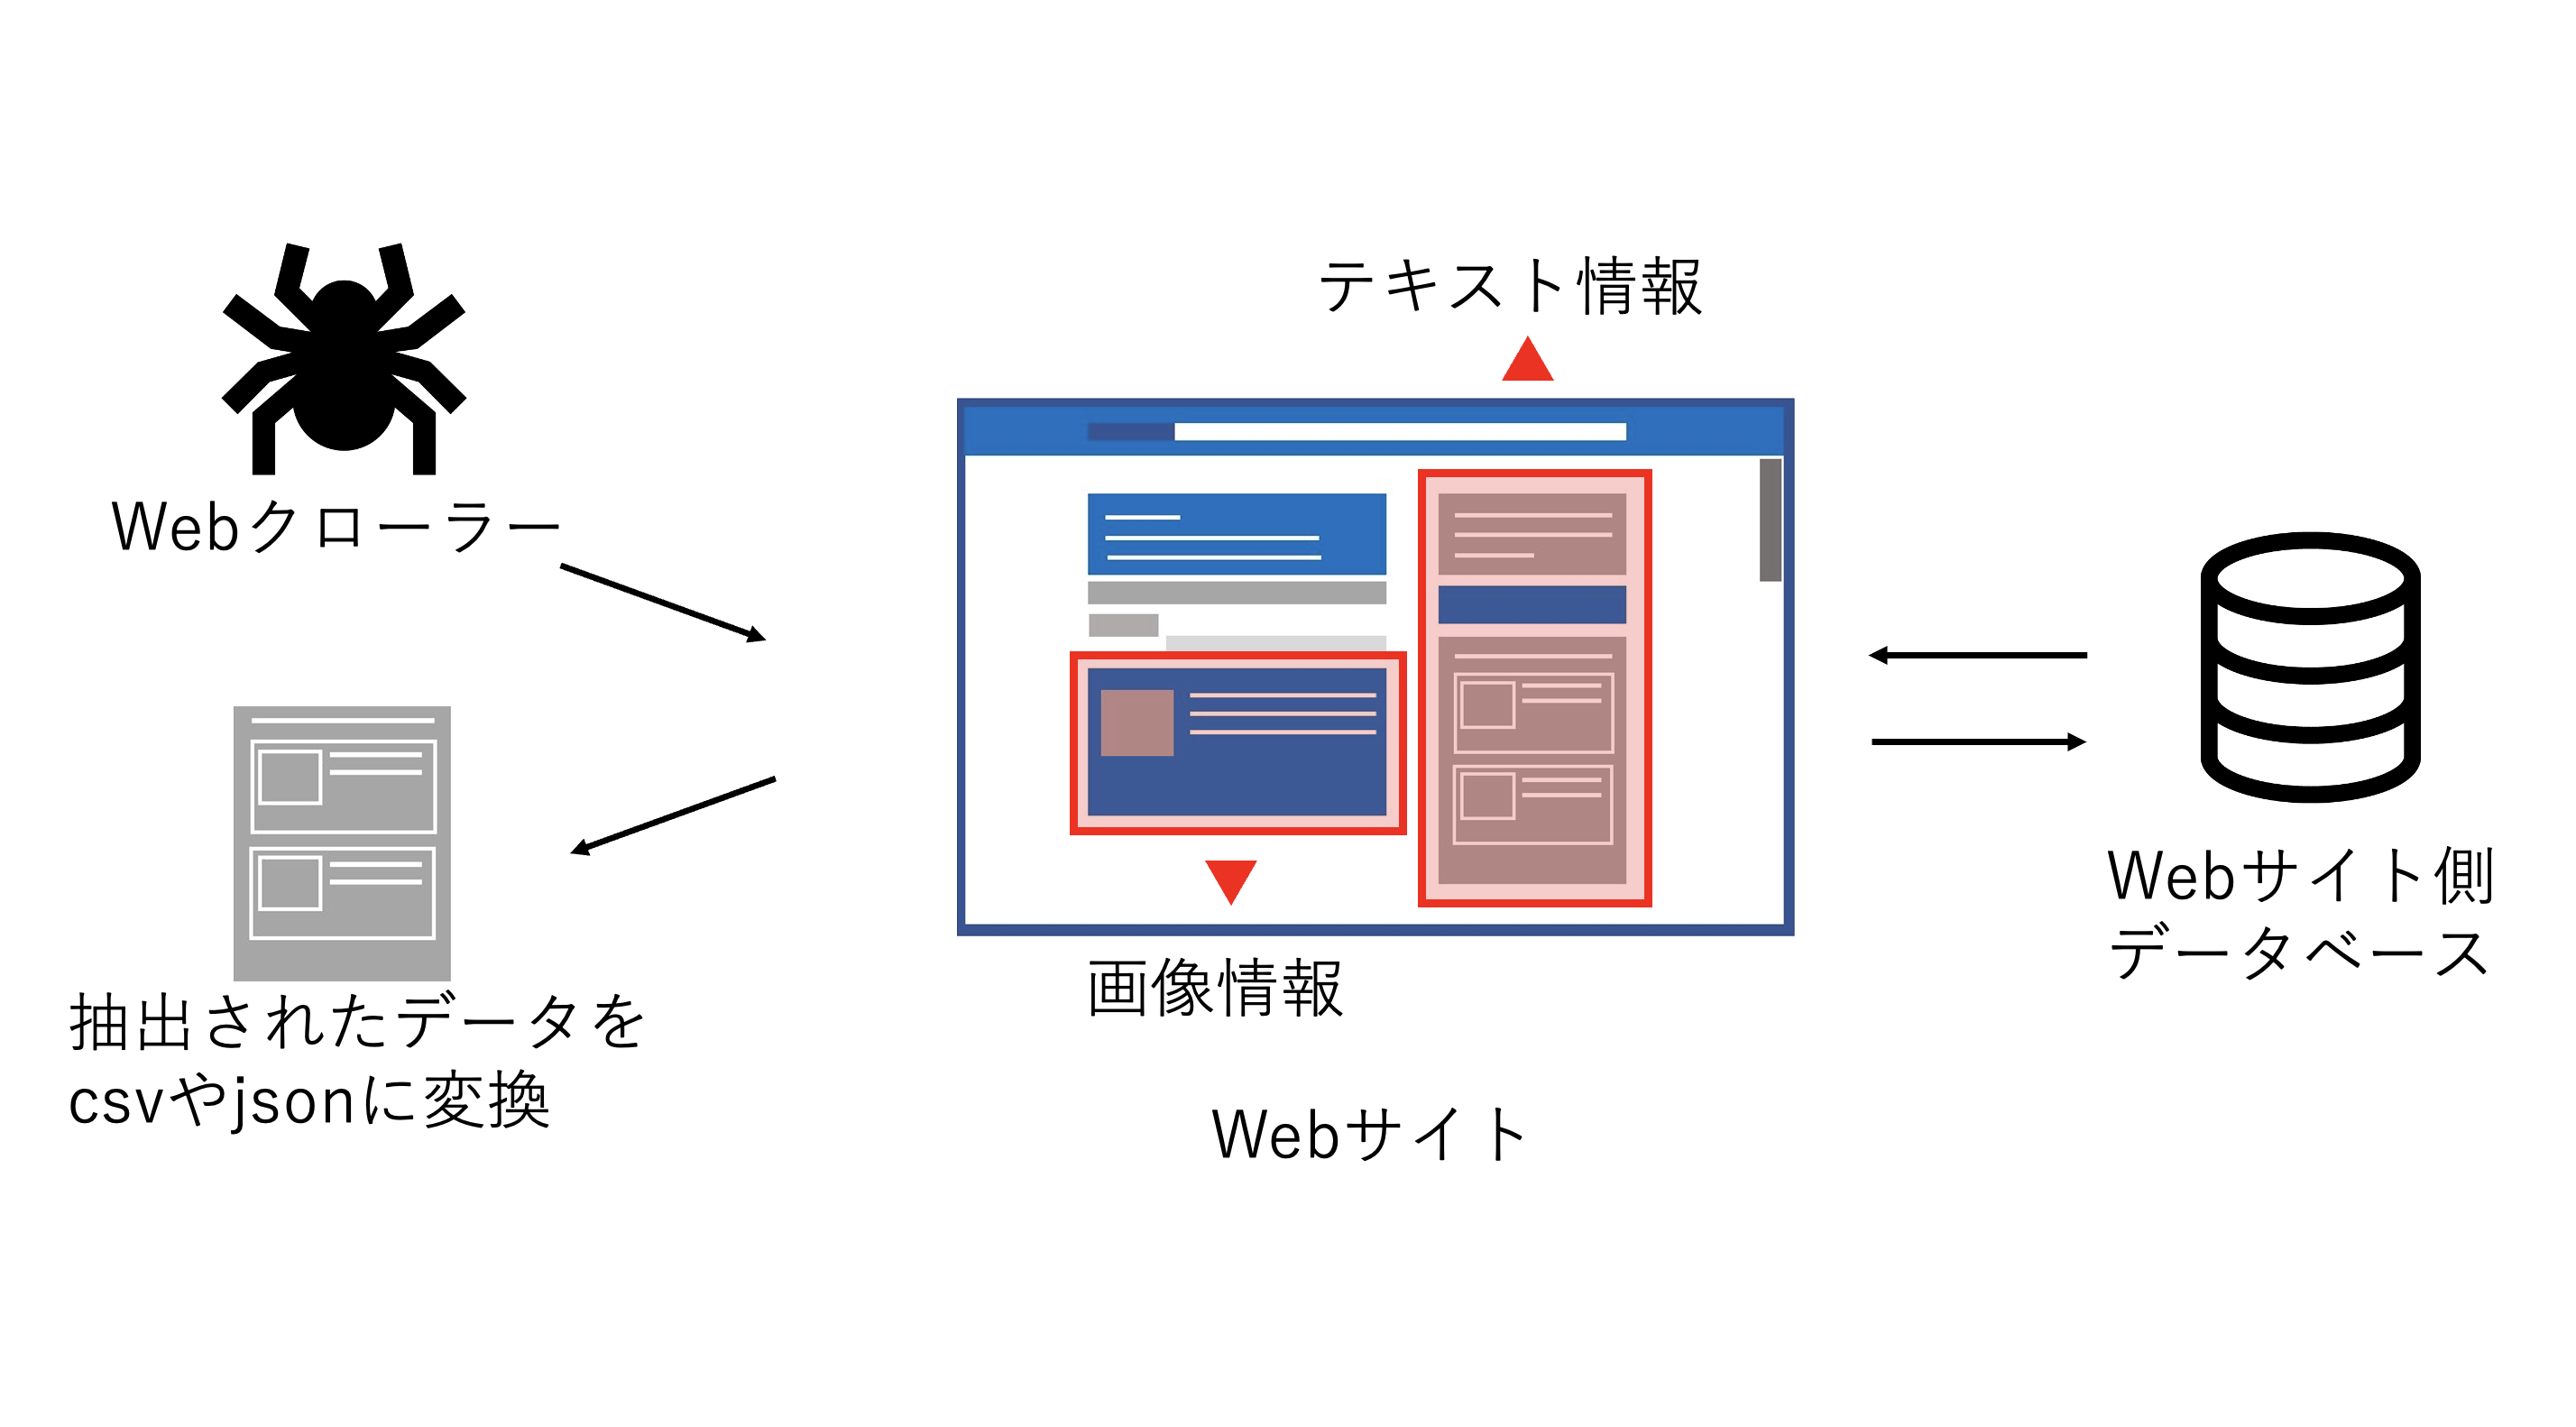
\includegraphics[width=0.9\linewidth]{./src/selenium.png}
	\caption{スクレイピングの解説}
  \label{fig:arch}
\end{figure}

\section{提案}

本研究では、スクレイピングを用いて未来大の学務情報をオープンデータとして提供し、情報到達容易性を向上させることである.

前述の通り、未来大の学務情報は現状複数のWebサイトに分散しているため、情報アクセスの効率が低下している.学務情報をオープンデータとして公開することによって、モバイルアプリなど他システムで活用できるようになり、情報の分散問題の解消や、情報アクセスの障害が低減することが期待される.
また、本提案のプラットフォームには、新たに”push型"の通知型メカニズムを導入する.これによって、現状学生が自主的に学務情報を取得しに行かなくてはいけない"pull型"から変更され、学生が自動的に通知を受け取る事ができ、情報の取得が効率的となる.この機能は学生が最新の情報にアクセスできるようにするための重要な要素である.


\section{実装}

本研究において、既存のWebサイトから学務情報を自動的に取得するためのスクレイピングツールとしてSeleniumを採用する.Seleniumは、動的なWebページやログインが必要なページの自動操作を得意とするブラウザ操作ツールである[1].このツールは、未来大の教務システムのような動的に内容の変わるWebページや、認証が要求されるページに置いて特に効果を発揮する.

システムの具体的な動作として、クライアントの要求を受け、Seleniumを使用して教務システムにログインし、学務関連の情報を取得する.対象とする情報は、大学からのお知らせ、学生個人の成績、時間割、休講、補講、教室変更、そして施設予約状況といった主要な項目を含む.取得したデータは、json形式に変換し、クライアントへレスポンスとして返送する.
さらに、取得した情報の利用を最大化するため、該当情報を中心としたモバイルアプリケーションの実装も行う.このアプリケーションにより、情報の一元化や、更新情報のpush型通知を行えるようにする.

また、本システムに置いてセキュリティの面で、取得した学務情報や学生の認証情報の安全性が最重要視される.そのため、サーバ側でこれらの情報を保存することは避けられており、代わりに情報は一時的なメモリ上でのみ取り扱われる方式を採用する.この情報はレスポンスが生成された直後に破棄される.特に、学生がシステムを利用する際のIDとパスワードといった認証情報の取り扱いは、さらなる注意が払われており、一度データが取得されると即座にメモリから削除する設計を施す.

\section{進捗状況}

ああああああ

\subsection{まとめ}


\subsection{情報システムコースにおける本研究の位置づけ}



\begin{thebibliography}{99}
	\bibitem{selenium}
	SeleniumHQ, "Selenium Documentation", Selenium, 2023. [Online]. Available from: \url{https://www.selenium.dev/documentation/en/}. Accessed: 2023-10-25.
\bibitem{marumaru}
	○○△△, システム情報科学会論文誌, 2, 13-19, 2002.
\bibitem{abc}
	A.B.Cdddddd, J. Systems Information Science, 11, 1145-1159, 2001.
\bibitem{batubatu}
	○○××, □□△△, システム情報科学, ☆☆出版, 1999, 20-21.
\bibitem{efghij}
	E.Fggg and H.Ijjj, Electrical Engineering, KKPress, 2003, 281-284.
\end{thebibliography}
\end{document}
%
%
% EOF 
